\documentclass[11pt, oneside]{article}  
\usepackage[margin=0.5in]{geometry} % Margins
\usepackage[ampersand]{easylist} % Bullets for lists
\usepackage[bottom]{footmisc}  % Glue footnotes to bottom
\usepackage{listings}
\usepackage{amsmath}
\usepackage{float}
\usepackage{array,mathtools}

\newcommand*{\carry}[1][1]{\overset{#1}}
\newcolumntype{B}[1]{r*{#1}{@{\,}r}}

\title{Homework 3\\UCLA-CS180-S18}
\author{Quentin Truong}


\begin{document}
\maketitle
\pagenumbering{arabic}


%========================================================
\section{Question 1}

Note: \newline
It has been clarified on Piazza that this graph may be disconnected and that this graph is undirected. \newline

Proof: \newline
We run BFS on each connected component to create the BFS tree.
We combine all the BFS trees together. Since they are disjoint, there will be no conflicts.
If the graph != combined bfs tree, then the graph must be have atleast one connected component with a cycle.
This is because a connected acyclic component is a tree, and a tree only has one possible spanning tree, itself.
We know any connected component without cycles must be a tree, and we know that each component is connected (by construction), and since the component is not a tree, it must have a cycle.
Since atleast one connected component has a cycle, the graph has a cycle. \newline

Algorithm: \newline
\begin{lstlisting}
function has_cycle(graph) // check if graph has cycle
    all_vertices = get_all_vertices(graph) // take all keys of adjacency list
    visited = []
    combined_bfs_tree = []

    if visited != all_vertices
        // then there is another connected component left
        unvisited = find_unvisited(all_vertices, visited)
        bfs_tree, discovered = create_bfs_tree(graph, unvisited)
        combined_bfs_tree += bfs_tree
        for vertex in discovered:
            if vertex == True
                visited.append(vertex)

    if is_equal(combined_bfs_tree, graph) // confirm that all edges in one are in both
        return false

    return true

function create_bfs_tree(graph, unvisited)
    discovered[unvisited] = True
    l = 0;
    levels[l] = [unvisited]
    while !level[l].empty()
        for vertex in levels[l]
            for neighbor of graph[vertex]
                if discovered[neighbor] != True
                    levels[l + 1].append(neighbor)
                    discovered[neighbor] = True
                    bfs_tree.add((vertex, neighbor))
        l += 1
    return bfs_tree, discovered

function find_unvisited(all_vertices, visited)
    for vertex in all_vertices
        if vertex not in visited
            return vertex

\end{lstlisting}

\clearpage
%========================================================

%========================================================
\section{Question 2}
\begin{figure}[ht]
\begin{center}
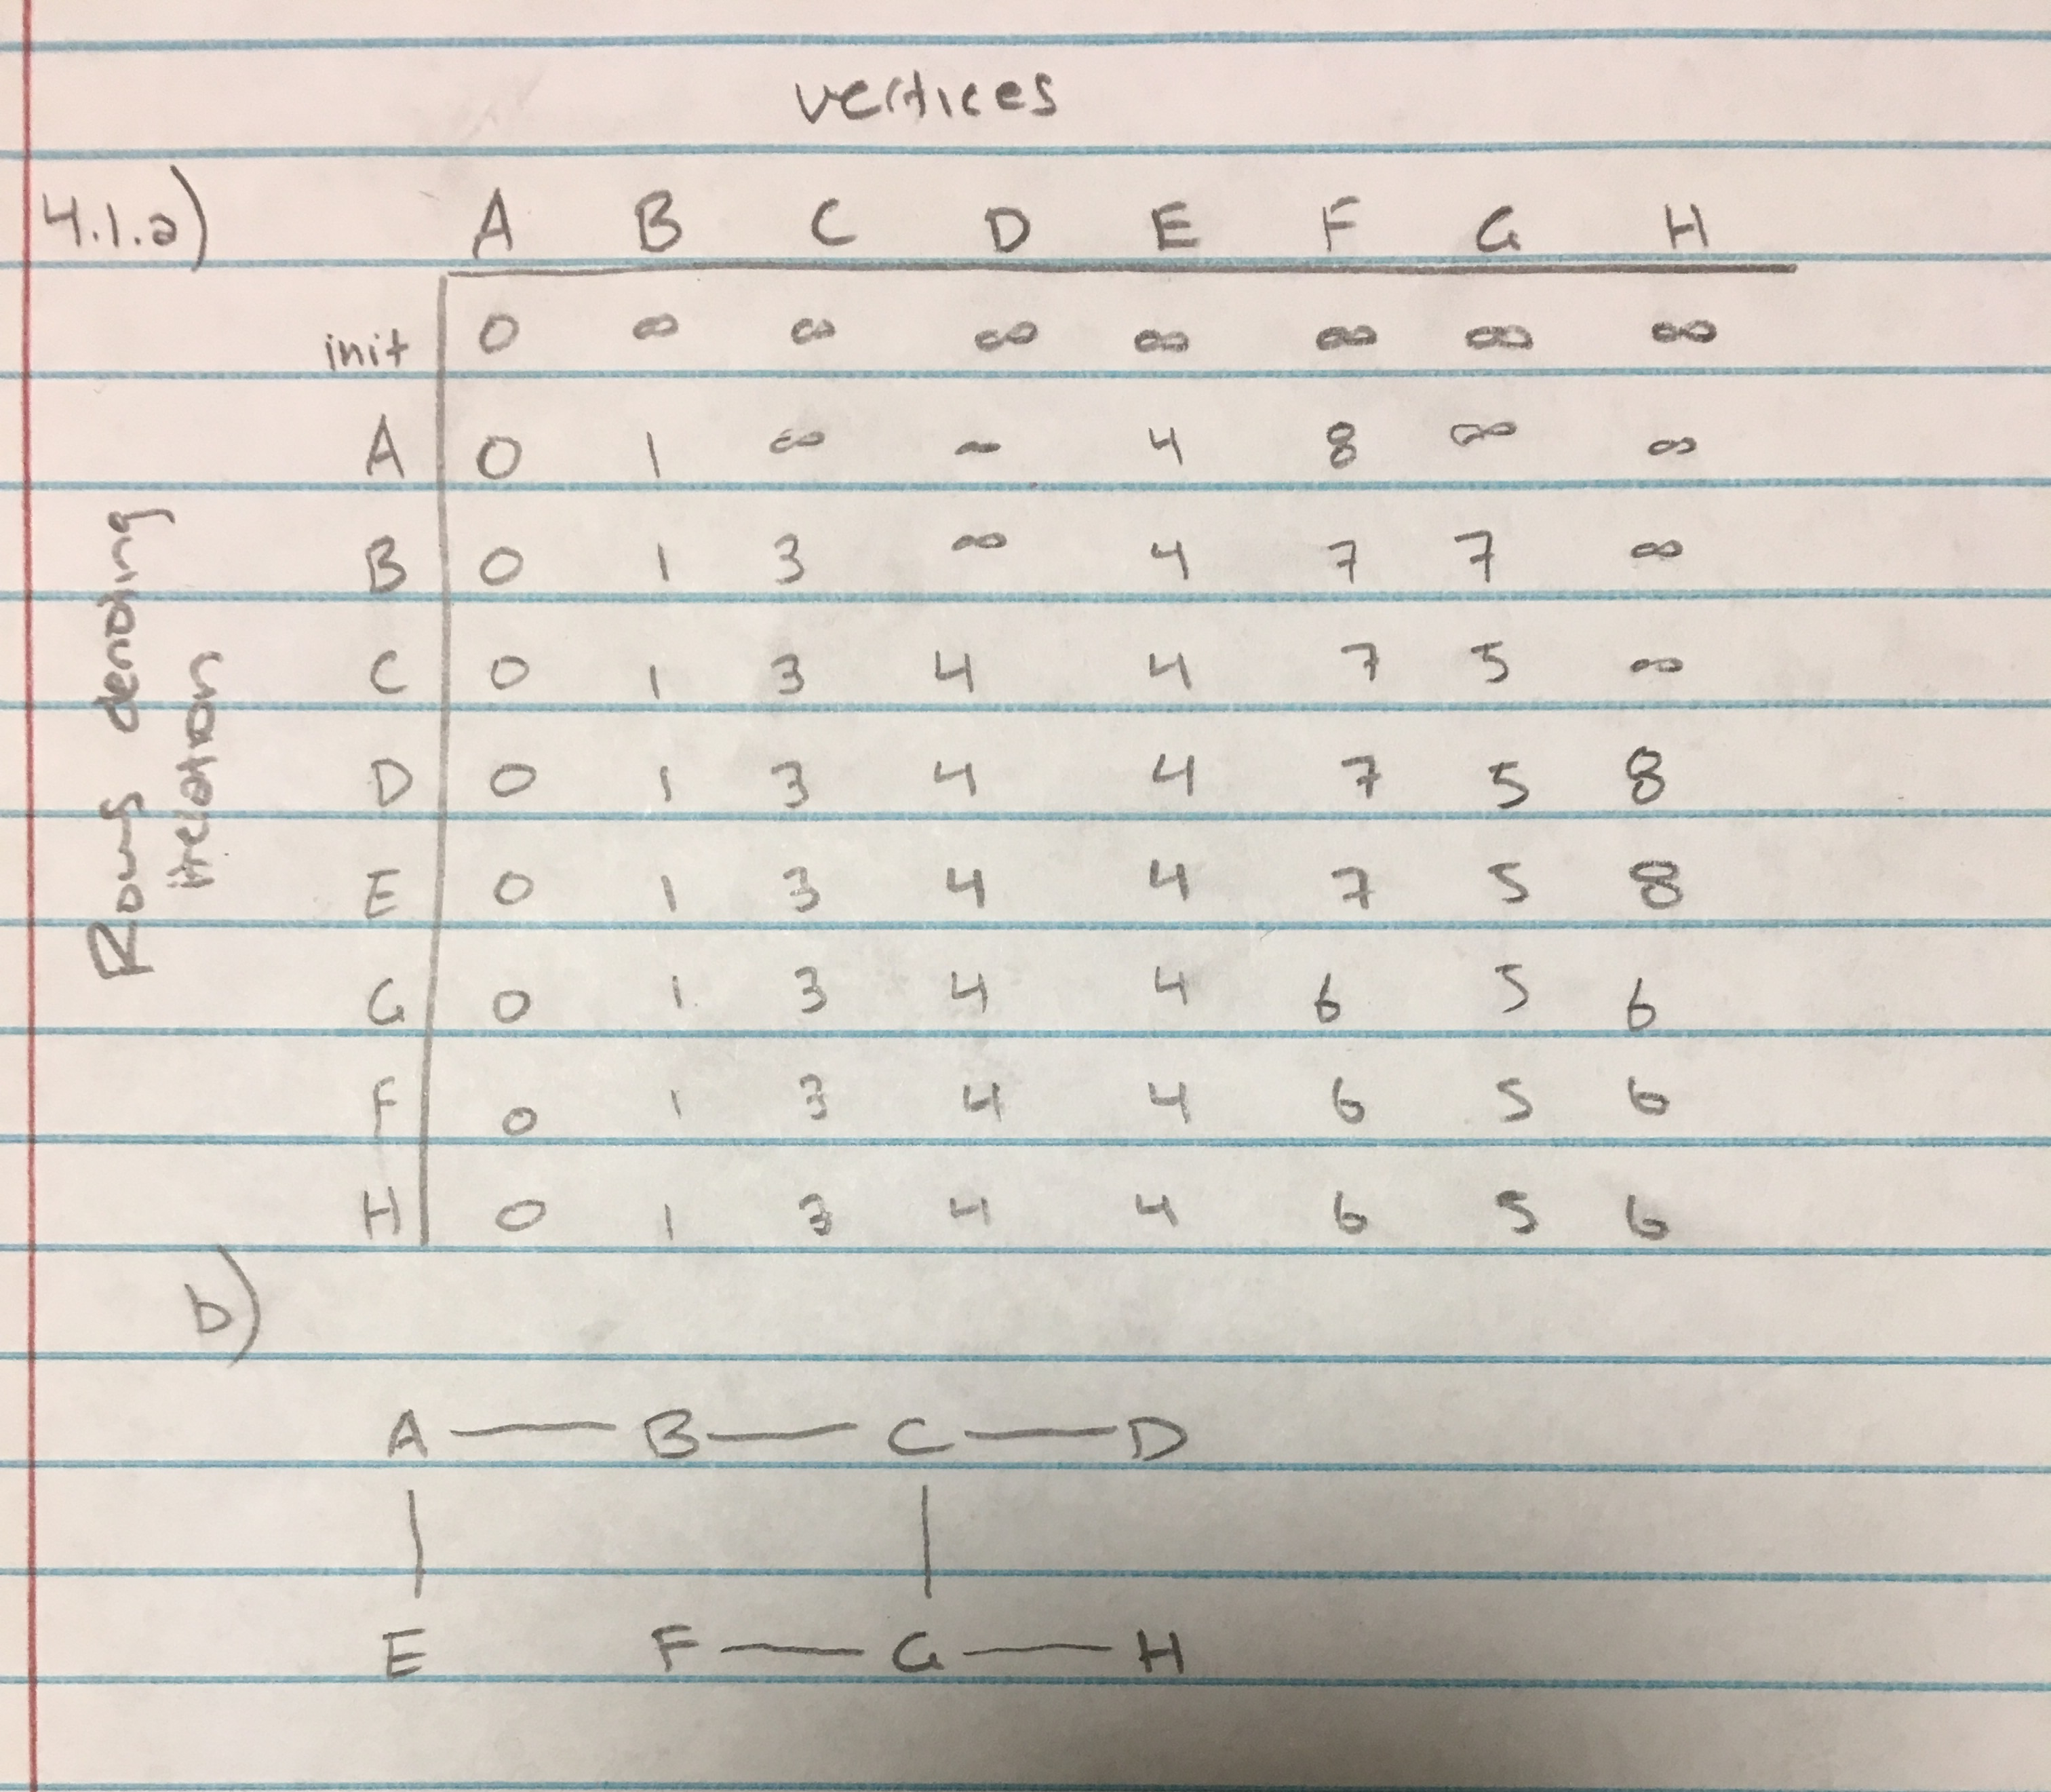
\includegraphics[width=\linewidth]{unnamed.jpg}
\end{center}
\end{figure}
\clearpage
%========================================================

%========================================================
\section{Question 3}

Intuition: Since the jobs from LST start later than or at the same time as the jobs from the optimal seqeuence, LST will always have enough time to do the same previous job as the optimal sequence. Therefore, LST is always at least as good as optimal. \newline

Lemma: LST picks jobs which start later than or at the same time as the optimal. \newline
Proof: (by induction) \newline
Suppose LST has jobs $A = [i_1, ..., i_n]$ \newline
Suppose optimal has jobs $A = [j_1, ..., j_n]$ \newline
Base: $l = n$ \newline
$i_n$ has latest start time, so is later than or as late as the optimal by definition \newline
Induction: \newline
Assume $i_l$ had latest start time \newline
start($j_{l-1}$) <= start($i_{l-1}$) < start($i_l$) because $i_{l-1}$ does not conflict with $i_l$ by definition \newline
So start($i_{l-1}$) is as late or later than start($j_{l-1}$) \newline

Theorem: LST produces the optimal sequence of jobs \newline
Suppose LST has jobs $A = [i_1, ..., i_n]$ \newline
Suppose optimal has jobs $A = [j_1, ..., j_n]$ \newline
We know that LST always picks jobs later than or at the same time as optimal, start($j_l$) <= start($i_l$). Therefore, LST will always have enough time to also choose any optimal previous job $j_{l-1}$. \newline

\clearpage
%========================================================

%========================================================
\section{Question 4}
Proof: \newline
Split T into its connected components.
The maximum independent set of T is equivalent to the combined maximum independent set of each connected component because each connected component is disjoint and thus fully independent from the others. \newline
Assume there is a maximum-size independent set S in a connected component of T which does not contain leaf node u. If S is size 1, there is only one node, so it must contain that node to be a maximum independent set. If S is size 2, both nodes are leaf nodes, and either may be picked to be a maximum independent set. If S is size 3, both leaf nodes must be picked to be a maximum independent size. If S is size 4 or greater, and a leaf node u is not picked, then a non-leaf node v connected to u must have been picked if it is a maximum independent set. If this is the case, we can replace node v with node u and obtain a new maximum independent set. This is because node u would be independent, because it is only connected to v, which was just removed. \newline

\begin{lstlisting}
function compute_independent_set_max_size(graph)
    independent_set = ()
    while graph.size() != 0
        edge = find_leaf_edge(graph) // (u, v), u is the leaf
        independent_set.add(edge[0])
        remove_edges(graph, edge[0]) 
        remove_edges(graph, edge[1])
    return independent_set

function find_leaf_edge(graph) 
    for i in range(0, graph.size())
        if graph[i].size() == 1
            return (i, graph[i][0])

function remove_edges(graph, vertex) 
    graph.remove(vertex) // remove any edge with vertex as source
    for i in range(0, graph.size()) // remove any edge with vertex as dest
        if vertex in graph[i]
            graph[i].remove(vertex)

\end{lstlisting}
\clearpage
%========================================================


\end{document}